\documentclass[conference]{IEEEtran}
\IEEEoverridecommandlockouts
\usepackage{cite}
\usepackage{amsmath,amssymb,amsfonts}
\usepackage{algorithmic}
\usepackage{graphicx}
\usepackage{textcomp}
\usepackage{xcolor}
\def\BibTeX{{\rm B\kern-.05em{\sc i\kern-.025em b}\kern-.08em
    T\kern-.1667em\lower.7ex\hbox{E}\kern-.125emX}}
\begin{document}

\title{Paper Title*\\
}


\author{\IEEEauthorblockN{Tugrul Yatagan\IEEEauthorrefmark{1} and
Sema F. Oktug\IEEEauthorrefmark{2}}
\IEEEauthorblockA{Department of Computer Engineering,
Istanbul Technical University\\
Istanbul, Turkey\\
Email: \IEEEauthorrefmark{1}yatagan@itu.edu.tr,
\IEEEauthorrefmark{2}oktug@itu.edu.tr}}
\maketitle


\begin{abstract}
Low power wide area network (LPWAN) technologies offer affordable connectivity to massive number of low-power devices distributed over very large geographical areas using license-free frequency bands. Focus on this work is one of the most promising LPWAN technologies: Lora. LoRa offers long range communication and strong resilience to interference by proprietary modulation technique based on Chirp Spread Spectrum (CSS). LoRa trades data rate for sensitivity and communication range by spreading symbols within a fixed channel bandwidth. SF assignment of nodes has strong effect on collisions thus network performance. In this work, we implemented a simulation environment to study different SF assignment schemes and we proposed a machine learning technique to optimize SF assignment. Finally, we illustrate simulation results for proposed machine learning SF assignment technique.
\end{abstract}


\begin{IEEEkeywords}
LoRa, Spreading Factor, IoT, LPWAN, Machine Learning
\end{IEEEkeywords}


\section{Introduction}
\par In the last few years, number of Internet of Things applications increase exponentially. \cite{7721743} Recent developments on LPWAN technologies has great impact on IoT application number growth. LPWAN technologies offer solutions to some of the oldest wireless communication challenges. Traditional wireless communication methods such as cellular networks (e.g., 2G, 3G, LTE) and short-range communication methods (e.g., Bluetooth, WiFi, Zigbee) cannot provide low power and long range at the same time. Cellular networks can provide long range and high data rate but they are complex and consume too much power. Besides, most of the IoT applications don't require high data rate. Short-range communication methods can provide relatively low power consumption but their range is limited to a few hundred meters at best. \cite{7815384} LPWAN technologies fill the technology gap between short range and cellular communication by providing low power and long range communication. LPWAN technologies basically sacrifice data rate to provide low power consumption.

\par There are several emerging LPWAN technologies. LoRa, SigFox, NB-IoT and LTE-M are commonly used, well known LPWAN technologies. LoRa and SigFox use license free ISM frequency bands while NB-IoT and LTE-M use licensed frequency bands which brings extra cost. Both LoRa and SigFox known for ultra low power consumption and resilient to interference while NB-IoT and LTE-M are promoted for higher data rate. 

LoRa has open standard MAC protocol called LoRaWAN.\\
LoRaWAN and SigFox use unslotted ALOHA based MAC protocol.\\
Private LoRaWAN networks can be deployed however SigFox and NB-IoT are operator based.\\
Sigfox limits the number of messages an end device can send (140 UL, 4 DL per day).\\
Sigfox payload is very limited 12 bytes UL and 8 bytes DL. LoRa 243 bytes, NB-IoT 1600 bytes.\\
Sigfox maximum data rate is also very low 100 bps, LoRa 50 kbps, NB-IoT 200 kbps.\\
LoRa can change data rate by spreading symbols within a fixed channel bandwidth. This enables tradeoff between sensitivity and data rate. LoRa has 7 different spreading factor option. Different spreading factor communications are orthogonal to each other.

\par TODO: SF Assignment Issue on LoRa

\par TODO: Proposal for SF Assignment Issue on LoRa

\par TODO: Organization of the paper


\section{Other Related Works}
\par TODO: Performance evaluation of lora networks in a smart city scenario\cite{7996384}

\par TODO: Scalability analysis of large-scale lorawan networks in ns-3 \cite{8090518}

\par TODO: Lora scalability: A simulation model based on interference measurements \cite{s17061193}

\par TODO: Impact of lora imperfect orthogonality: Analysis of link-level performance \cite{8267219}

\par TODO: Scalability analysis of a lora network under imperfect orthogonality \cite{8430542}


\section{LoRa}
\par LoRa is the name of the physical layer Radio/Chipset technology that provides wireless link for low power wide area networks. LoRa uses proprietary spread spectrum modulation technique that is derivative of Chirp Spread Spectrum (CSS). LoRa is registered trademark of Semtech Corporation. LoRa has an open standard MAC protocol called LoRaWAN. LoRa and LoRaWAN terms are frequently and incorrectly used for each other.

\subsection{LoRaWAN}
\par LoRaWAN is a media access control (MAC) layer protocol which designed for large scale LoRa networks. LoRaWAN is an open source standard developed and maintained by LoRa Alliance. LoRa Alliance is an open, non-profit organization dedicated to promoting the interoperability and standardization of LoRaWAN. LoRa can be used without LoRaWAN as a wireless link technology, however LoRaWAN is developed considering well known LPWAN challenges and their best practice solutions. LoRaWAN also provides interoperability between different networks. LoRaWAN uses unslotted ALOHA to access medium. LoRaWAN provides lightweight but powerful standard for IoT applications.

\par TODO: explain end node, gateway, class A

\subsection{LoRa Modulation}
\par TODO

\subsection{Spreading Factor}
\par LoRa CSS modulation can spread the symbols.\\
The spread factor is the ratio between symbol rate and chip rate. The ratio between symbol and chip rate is $2$\textsuperscript{spreadfactor}.\\
Six different spread factors are available (between 7 and 12); increasing the spread factor makes the signal more robust to noise, but decreases the data rate.\\

\par Lowest SF suitable area section is relatively higher then the others. Most of the end devices which close to GW will fall into this area. Figure~\ref{fig:problem1}

\par End devices near the GW will probably select lowest SF all the time. Which results a lot of collisions between lowest SF transmissions while end device number near the GW increases. Figure~\ref{fig:problem2}

\begin{figure}
\centering
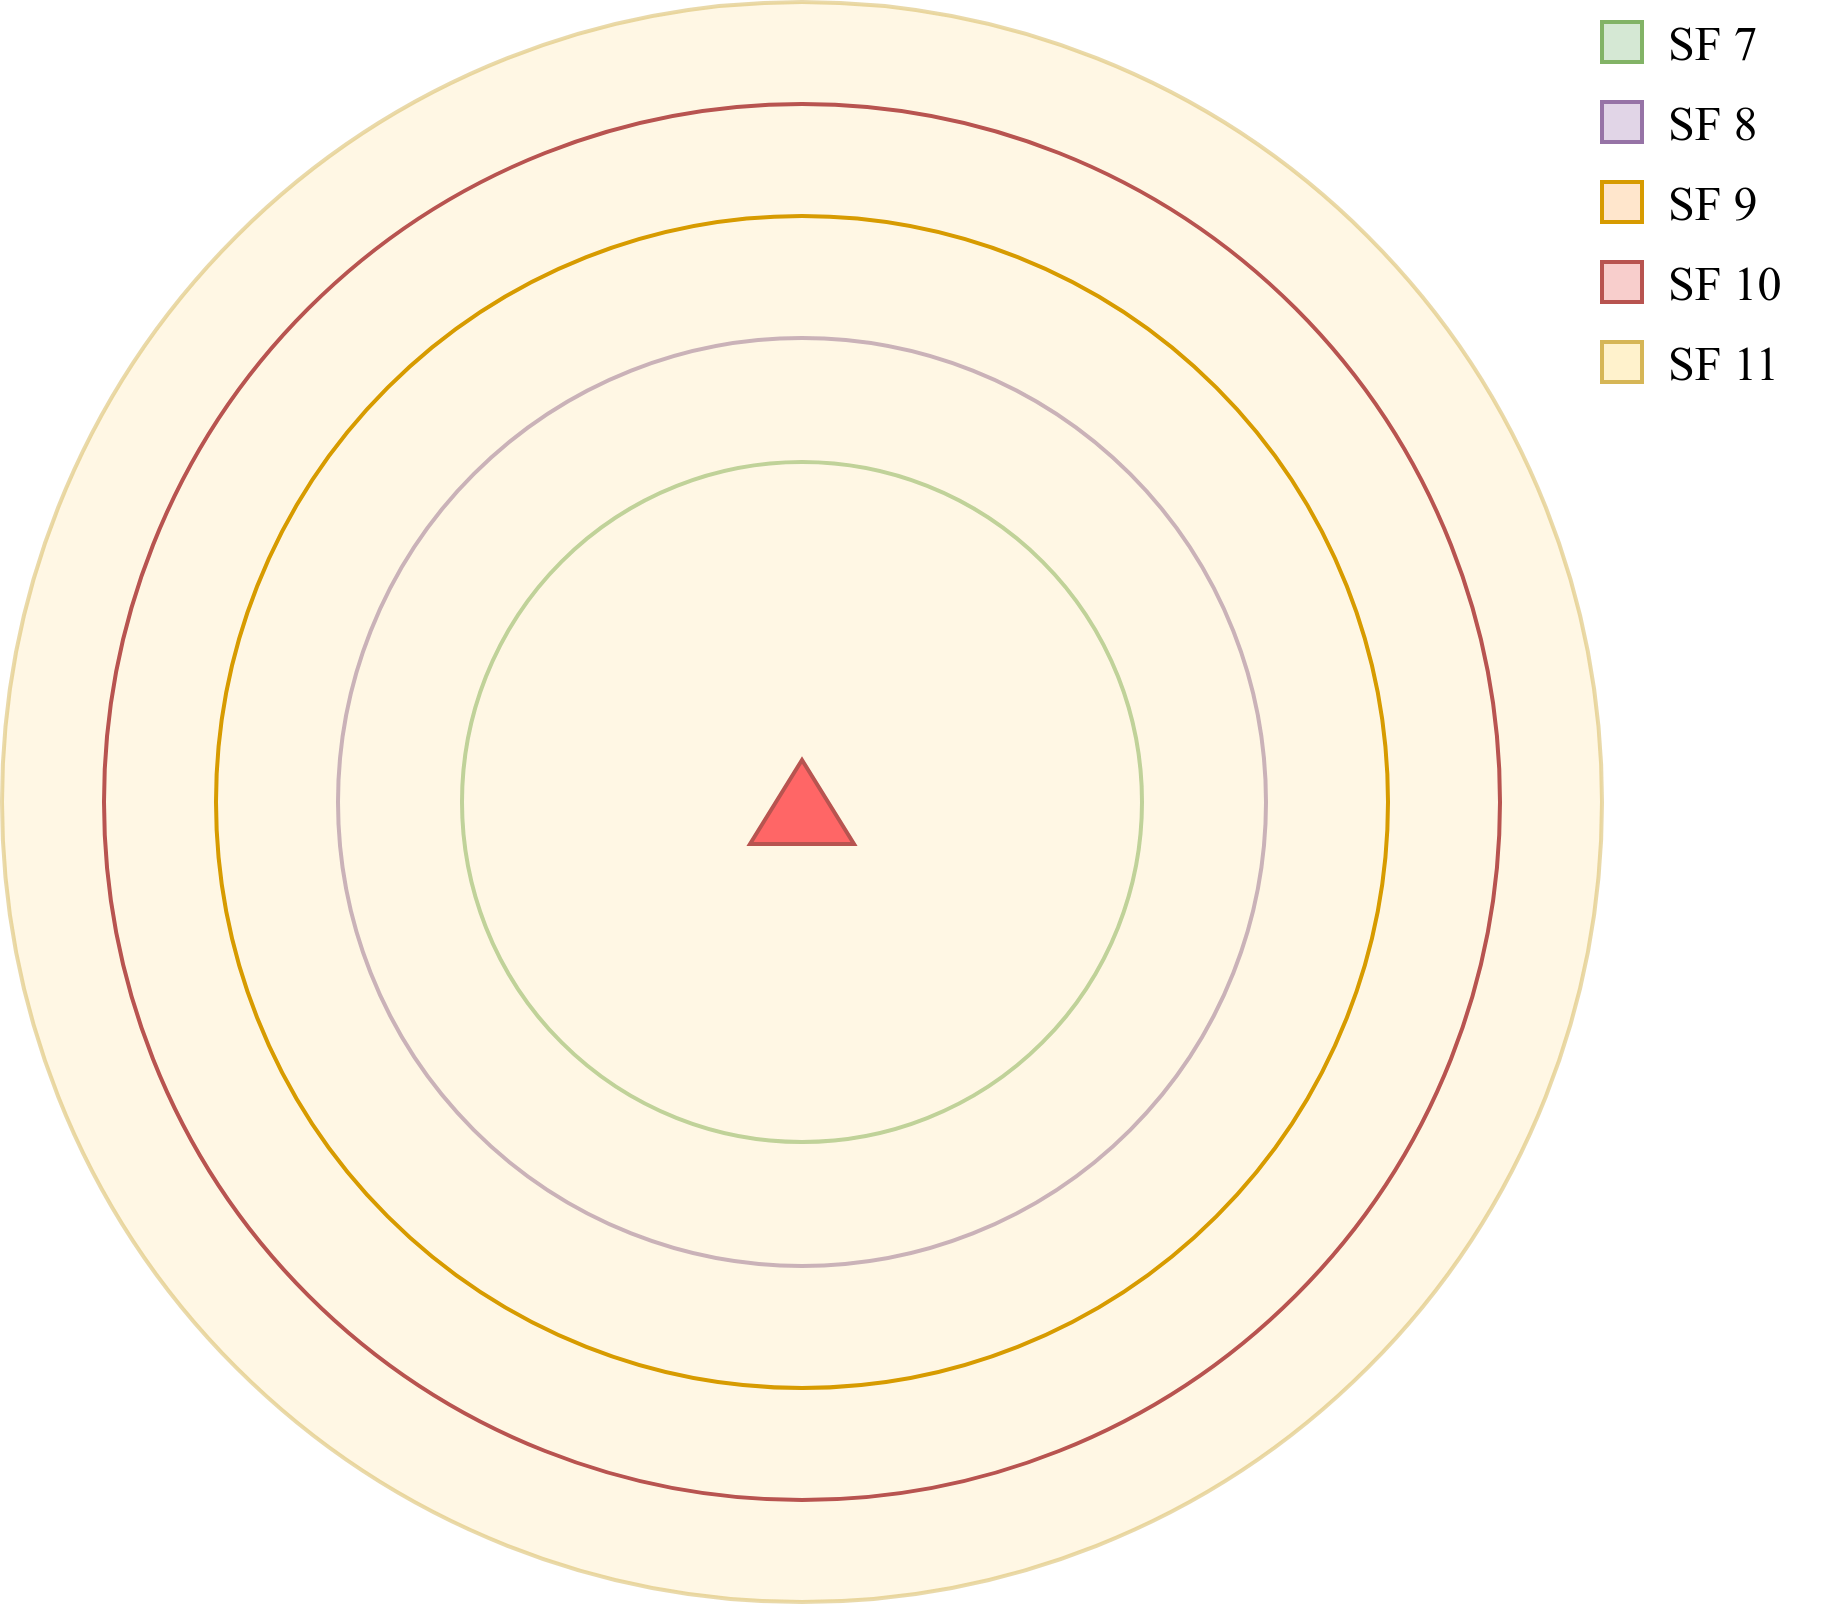
\includegraphics[width=0.5\textwidth]{lora0-1}
\caption{Different SF ranges.}
\label{fig:problem1}
\end{figure}

\begin{figure}
\centering
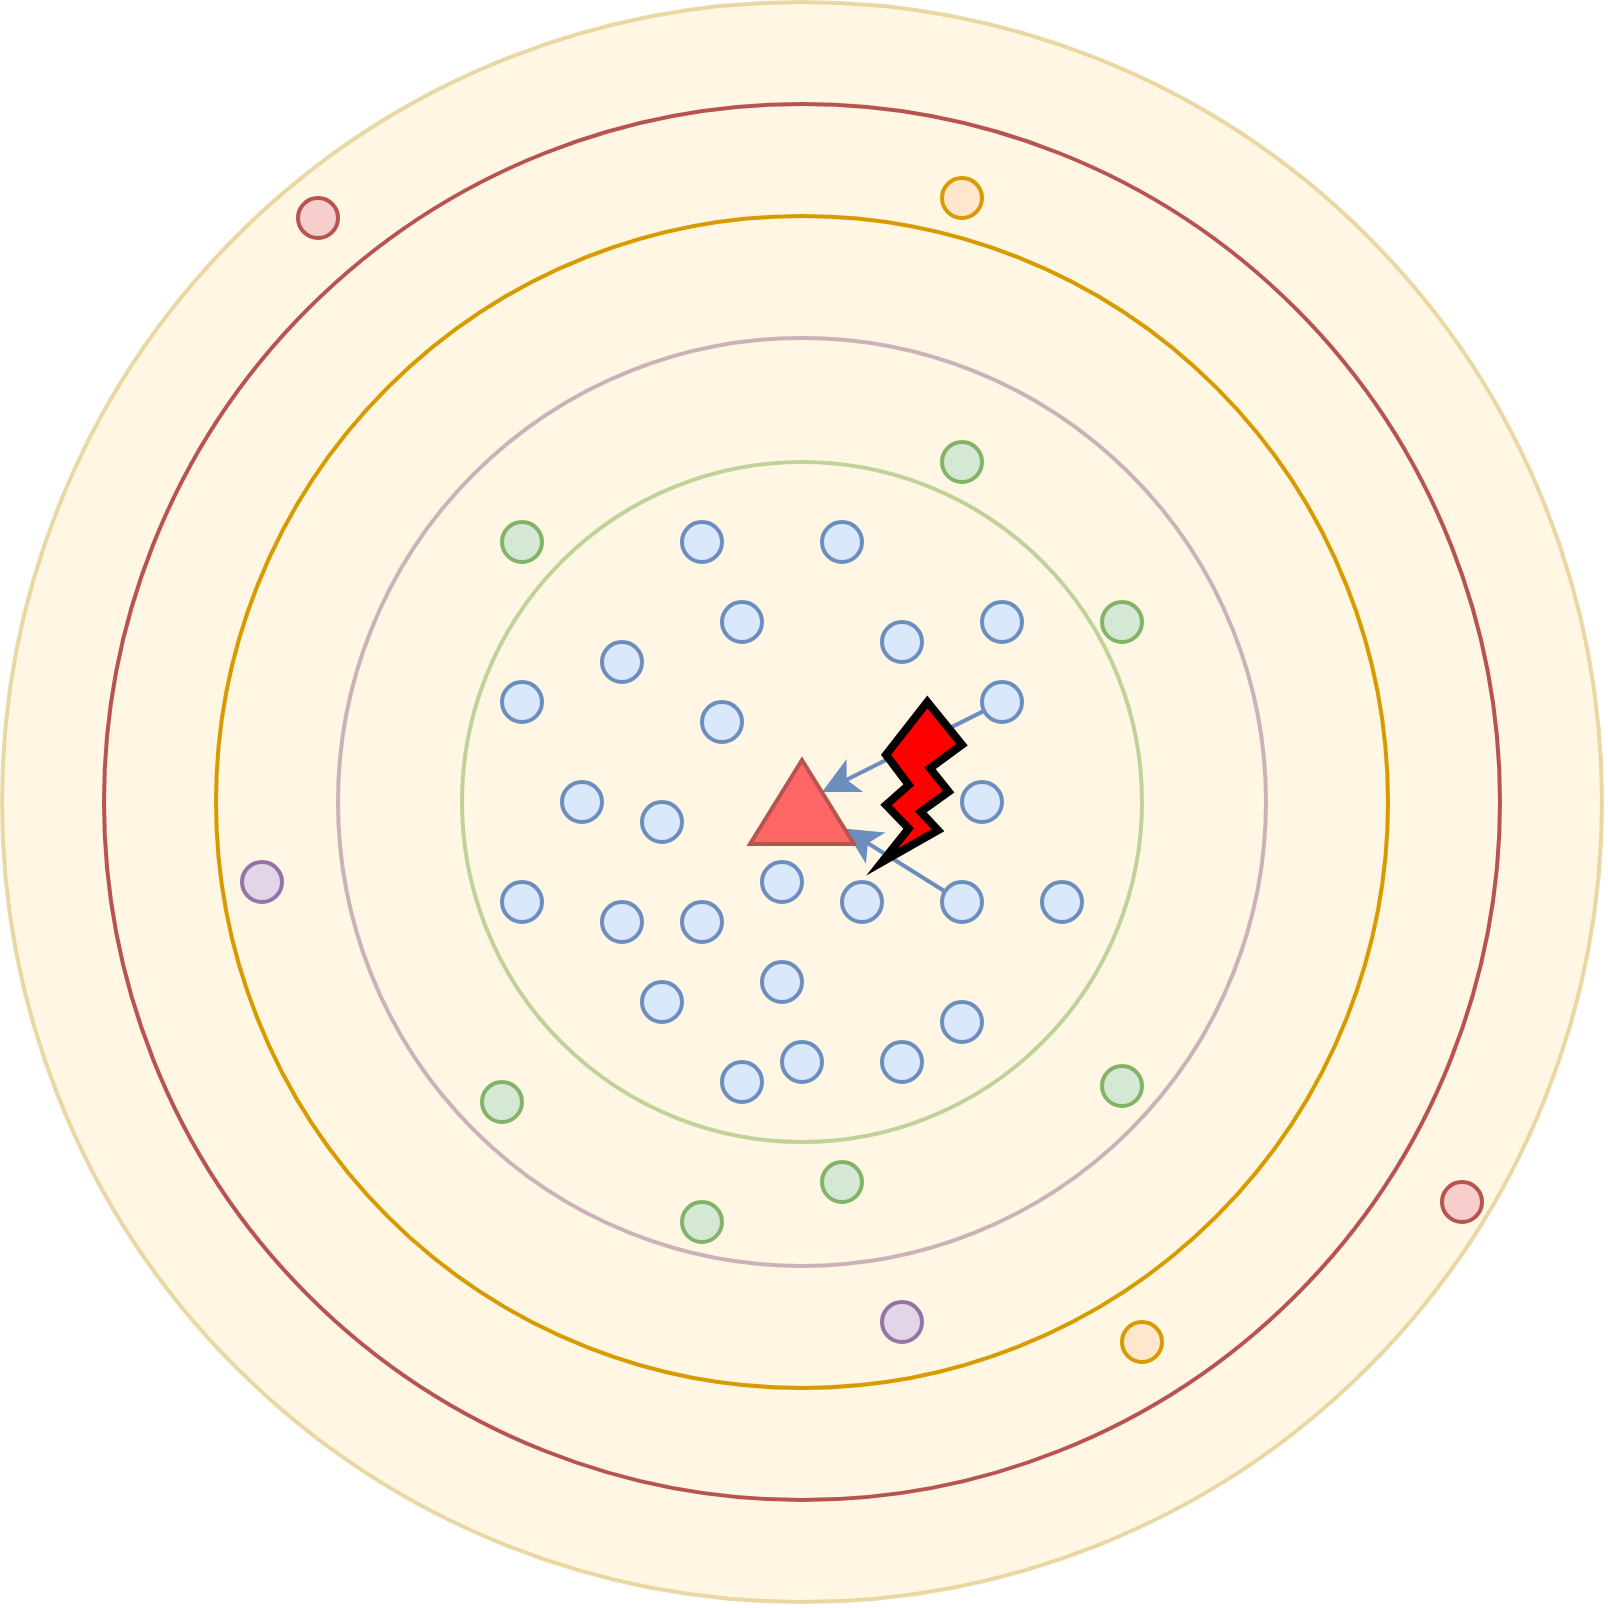
\includegraphics[width=0.5\textwidth]{lora1-1}
\caption{Collision between nodes near the GW.}
\label{fig:problem2}
\end{figure}


\section{Proposed Technique}
\par If GW force some of close end nodes to select higher SF even if they can able to communicate with lower SF, this will result lower collisions due to the orthogonality of different SF. Figure~\ref{fig:proposal_single_gw}

\par GW can avoid increasing SF of end nodes which is close to other GW using location information obtained by triangulating the signal strength of end nodes. Figure~\ref{fig:proposal_multi_gw}

\begin{figure}
\centering
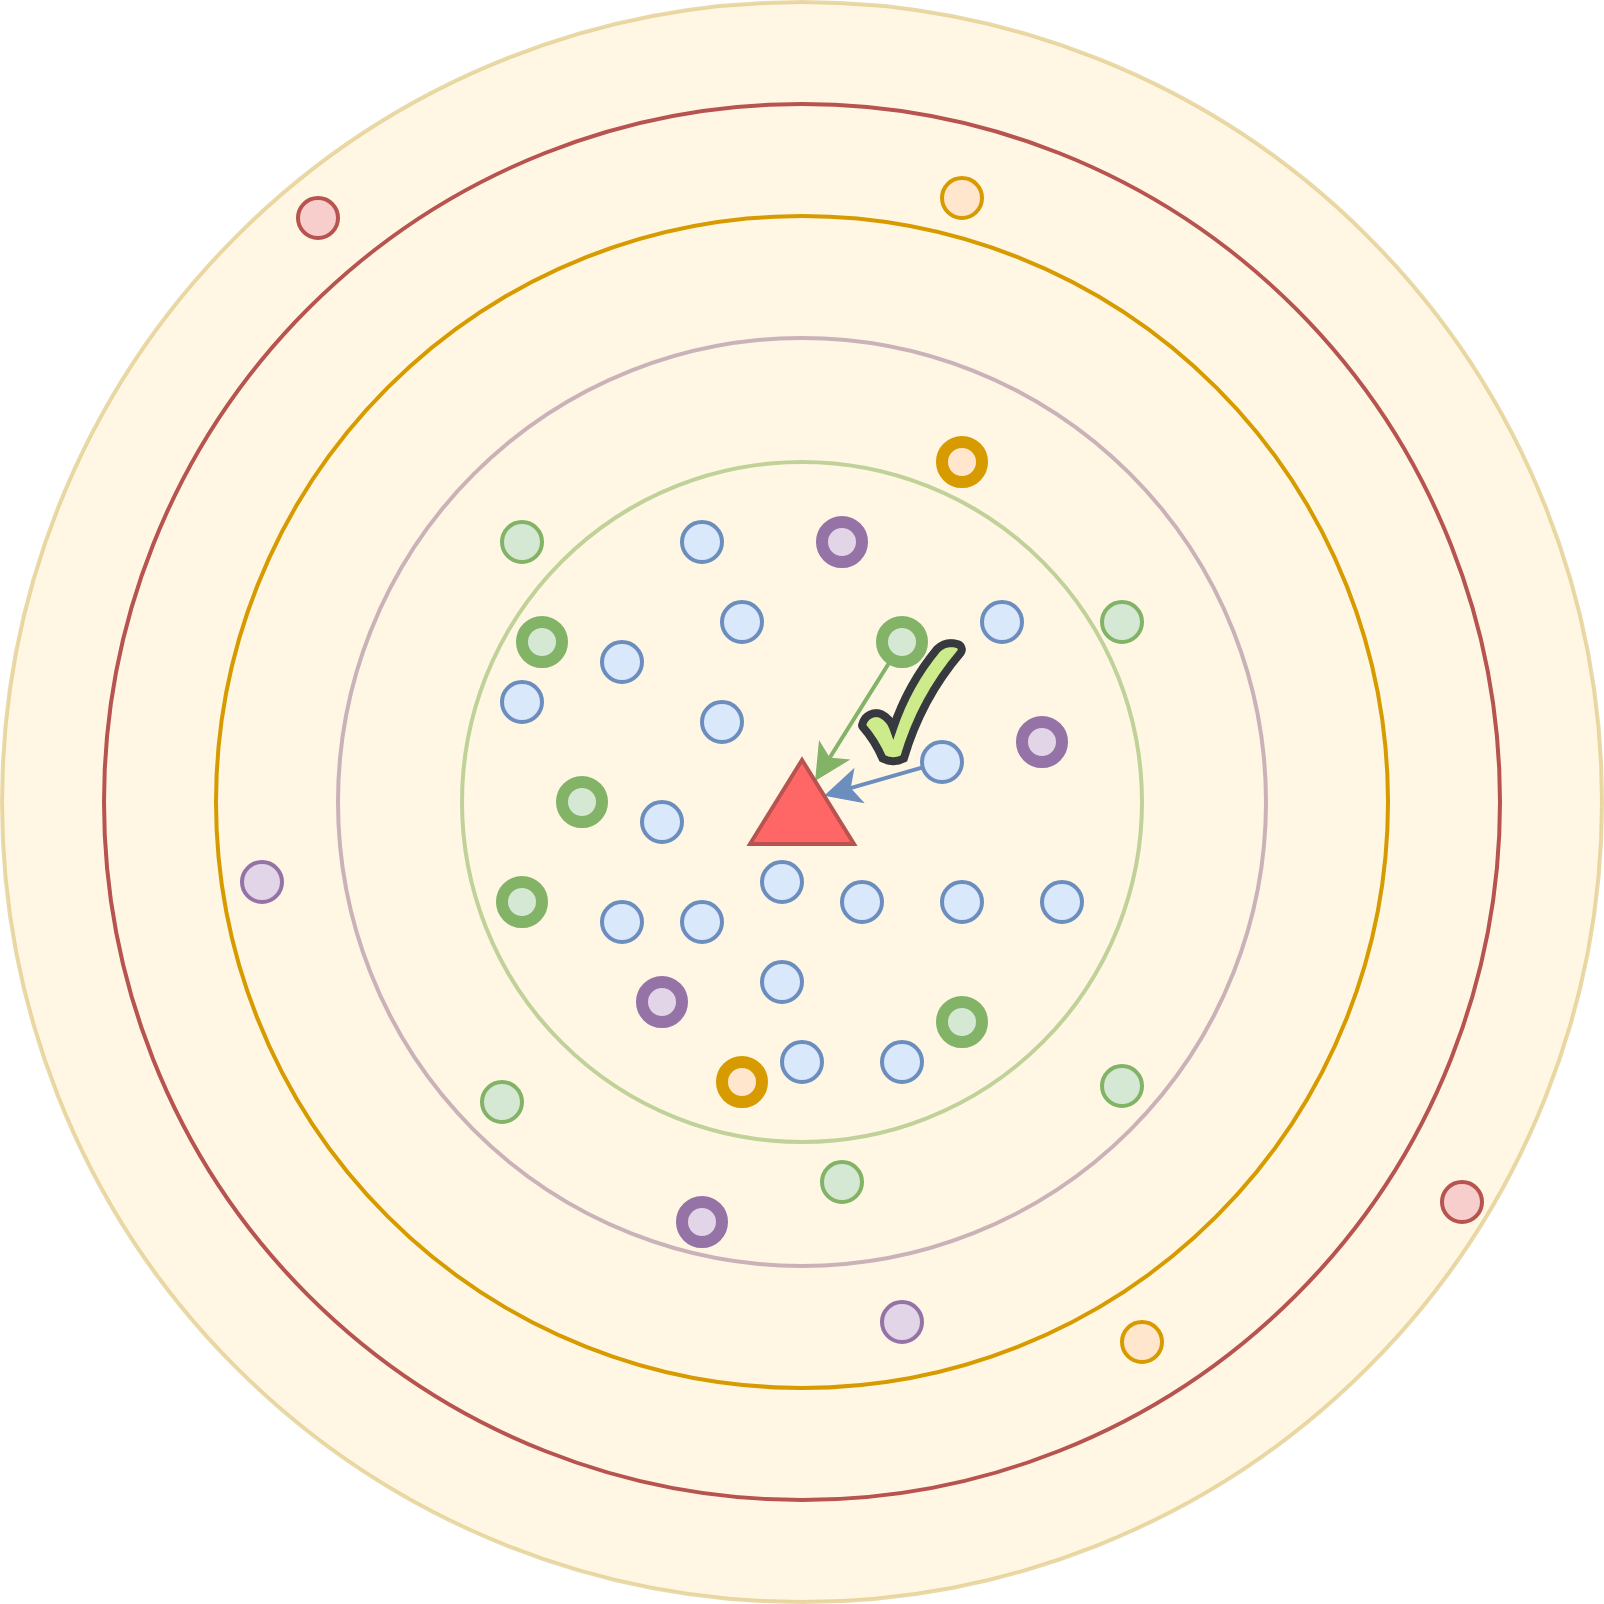
\includegraphics[width=0.5\textwidth]{lora2-1}
\caption{Collision between nodes near the GW can be prevented by using higher SF.}
\label{fig:proposal_single_gw}
\end{figure}

\begin{figure}
\centering
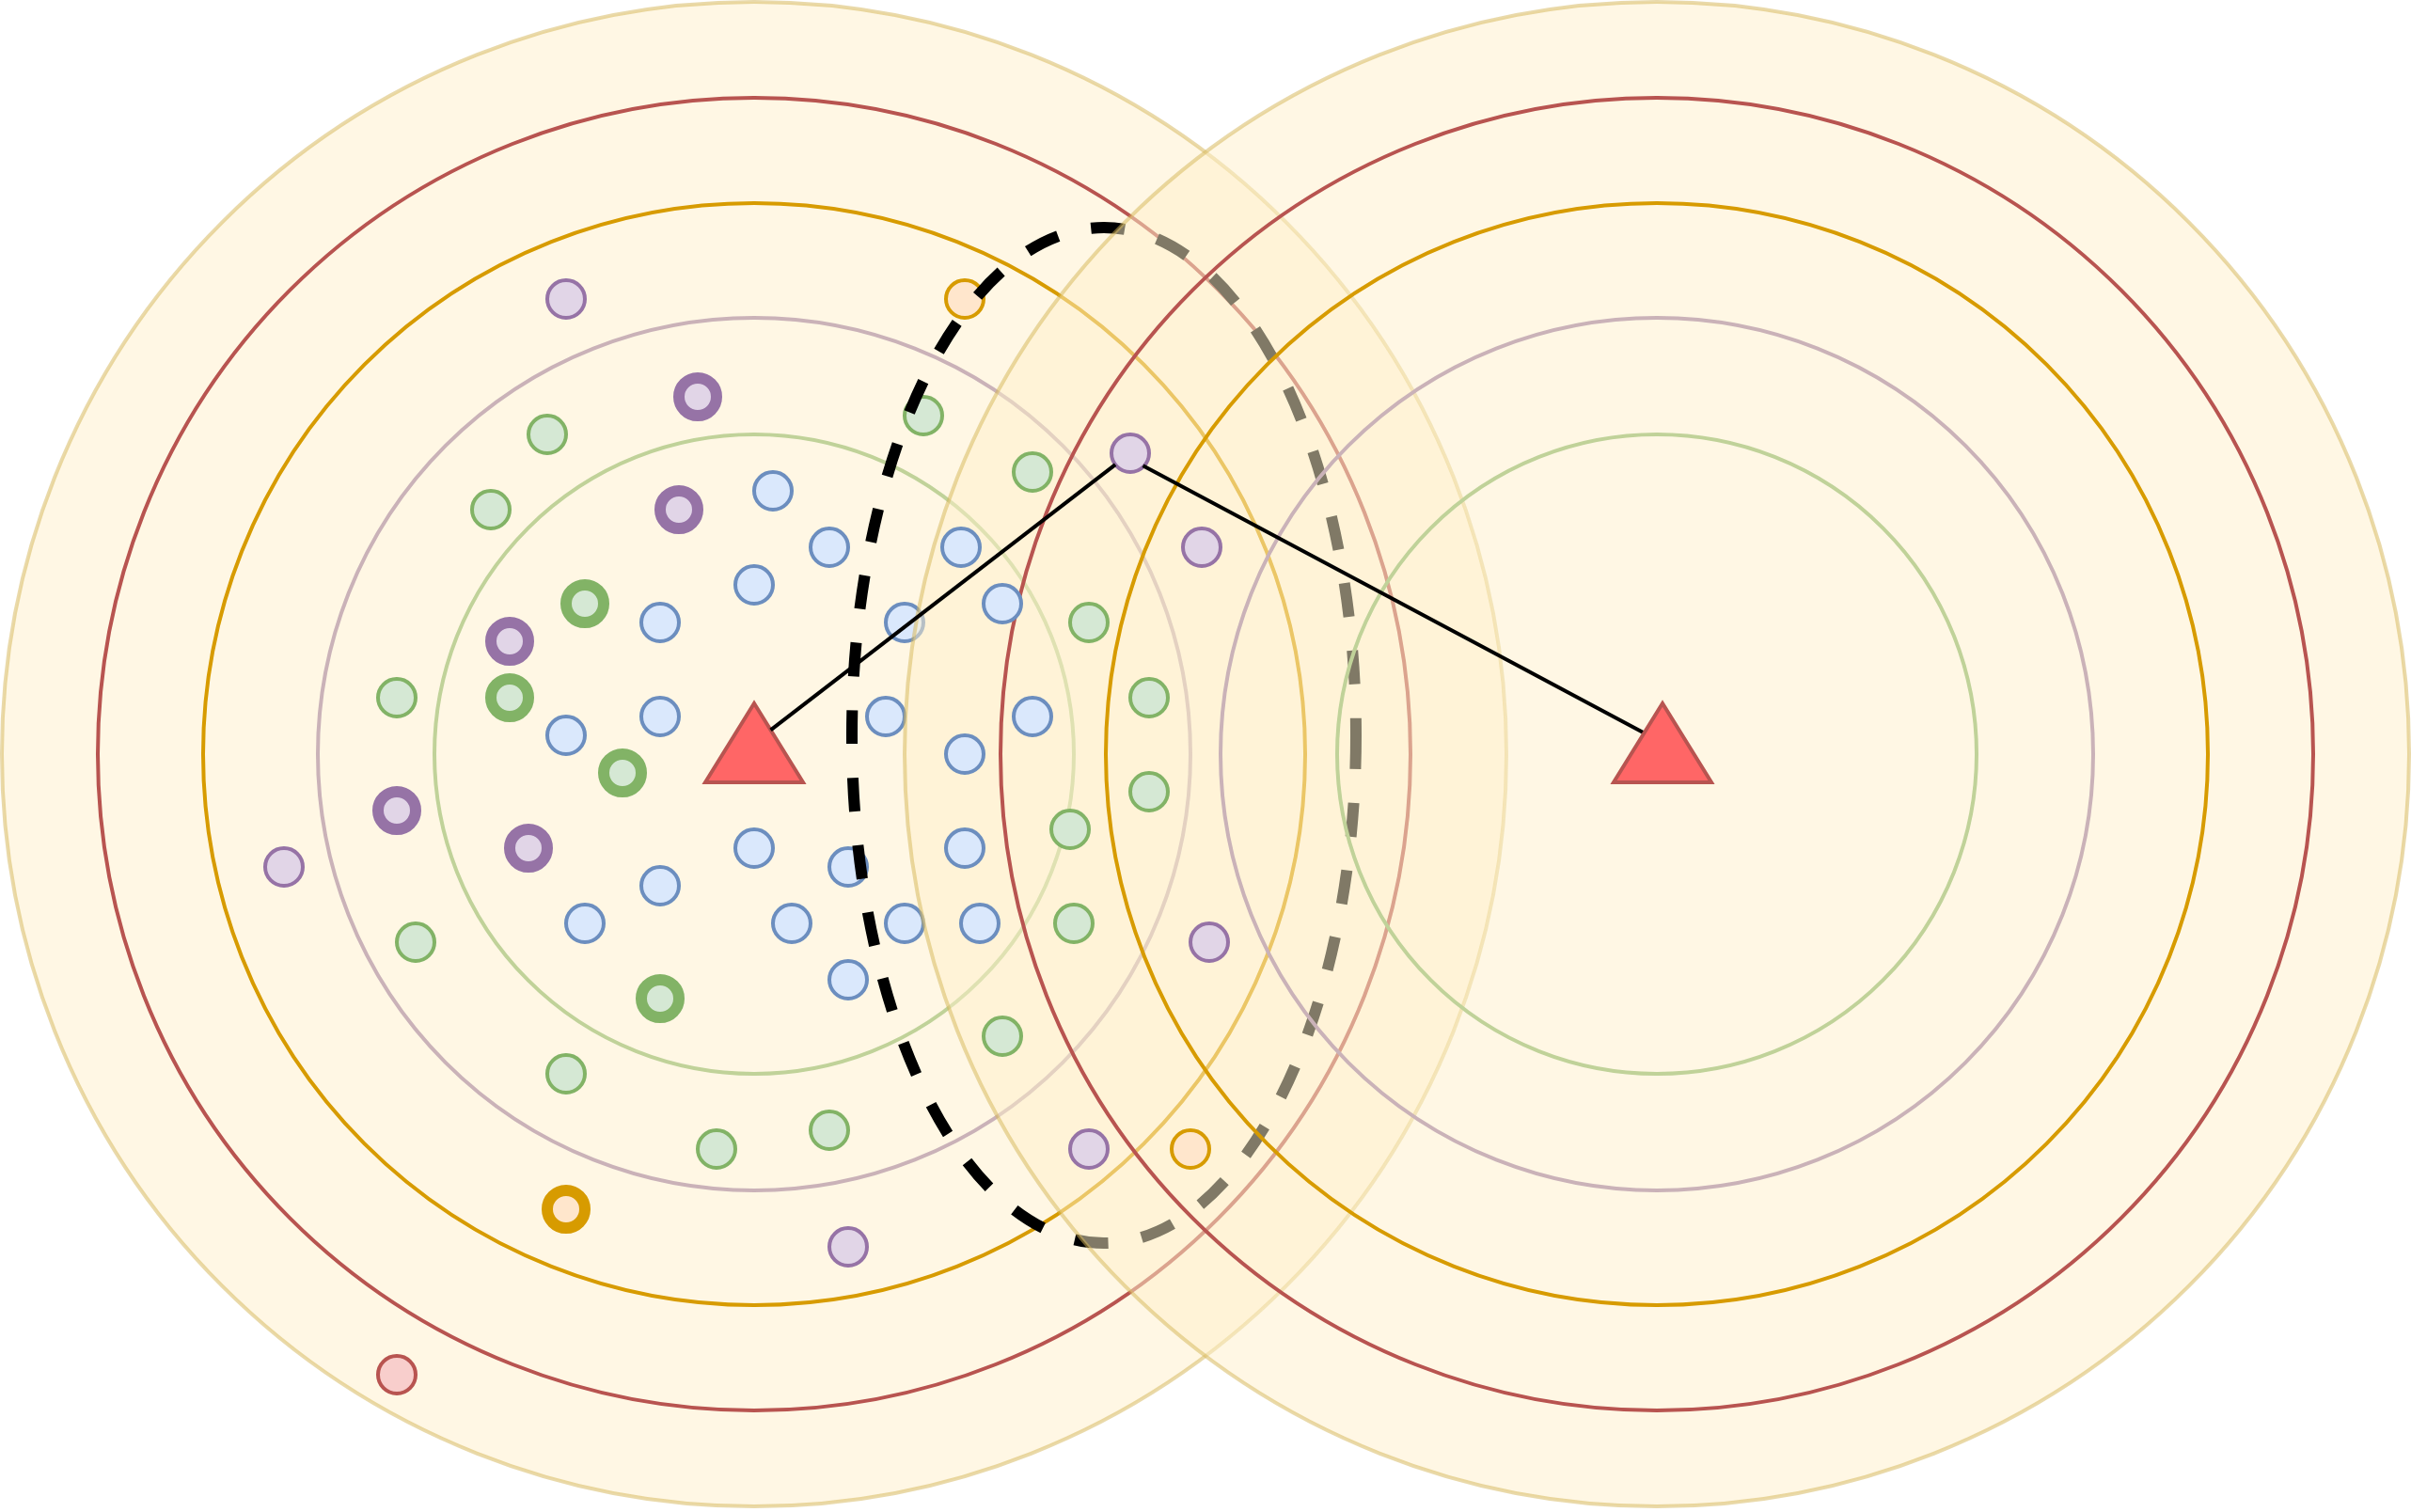
\includegraphics[width=0.5\textwidth]{lora3-1}
\caption{Collision prevention proposal for intersecting GWs.}
\label{fig:proposal_multi_gw}
\end{figure}


\section{Simulation Environment}
A discrete event simulator is implemented in Python to simulate LoRa network performance. 
https://github.com/tugrulyatagan/simlorafs

\subsection{Link Model}
TODO

\subsection{Interference Model}
TODO

\subsection{Simulation Assumptions}
TODO

\begin{figure}
\centering
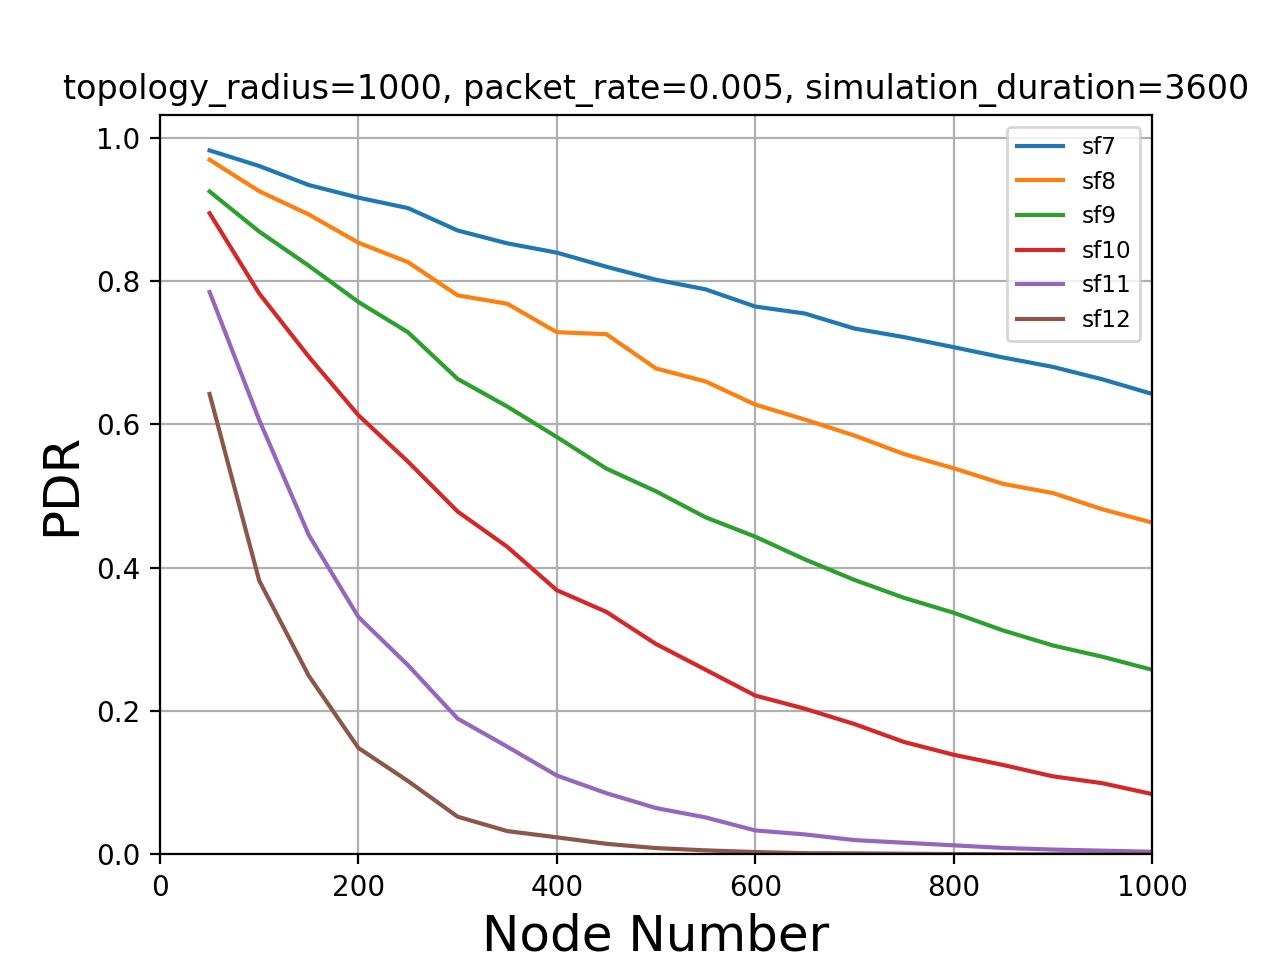
\includegraphics[width=0.5\textwidth]{sf_1000}
\caption{PDR of different SF when radius is 1000m.}
\label{fig:sf_1000}
\end{figure}

\begin{figure}
\centering
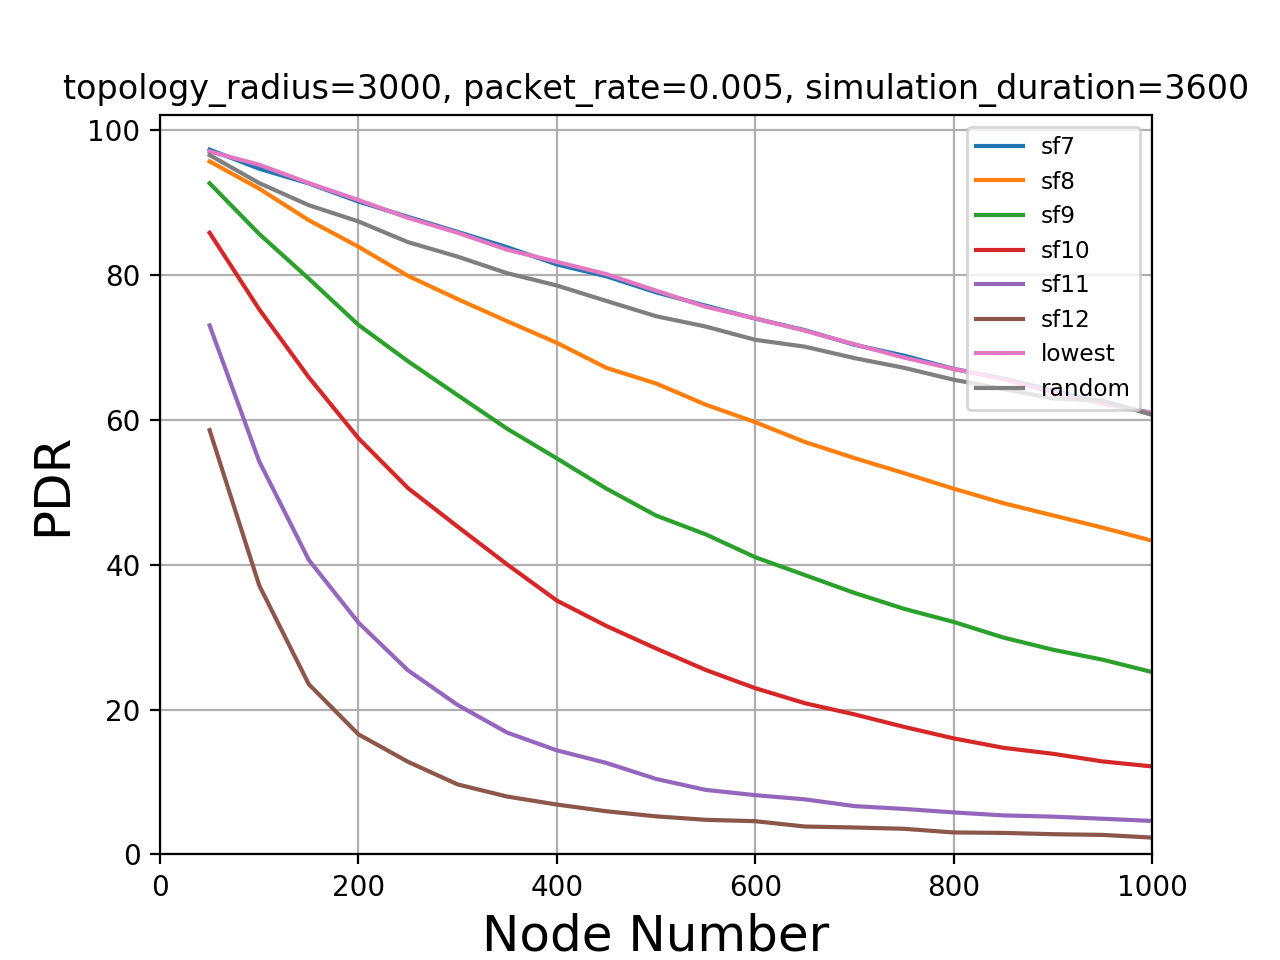
\includegraphics[width=0.5\textwidth]{sf_3000}
\caption{PDR of different SF when radius is 3000m.}
\label{fig:sf_3000}
\end{figure}

\begin{figure}
\centering
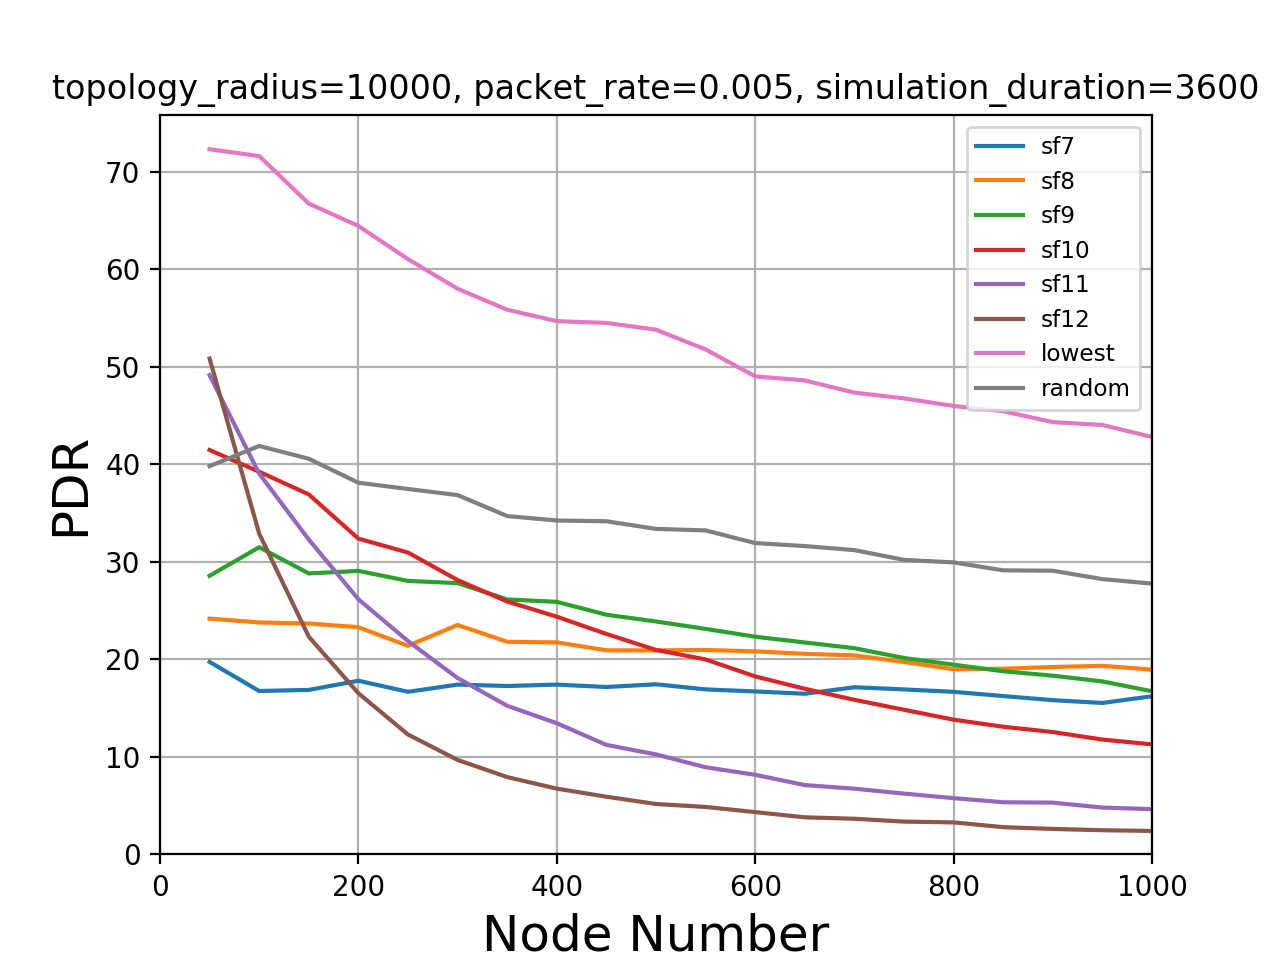
\includegraphics[width=0.5\textwidth]{sf_10000}
\caption{PDR of different SF when radius is 10000m.}
\label{fig:sf_10000}
\end{figure}


\section{Simulation Results}
TODO: Evaluation


\section{Conclusion}
TODO: Summary, future works
\cite{7815384} \cite{7803607} \cite{7996384} \cite{8090518} \cite{s17061193} \cite{8267219} \cite{8430542} \cite{8319183} \cite{8480649} \cite{AN1200.22} \cite{Bor:2016:LLW:2988287.2989163} \cite{8406255} \cite{DBLP:journals/corr/abs-1802-10338} \cite{finnegan2018comparative}


\section*{Acknowledgment}
This work is supported by Turkish Ministry of Development and Istanbul Technical University researcher support program under the Grant No. ITU-AYP-2017-1. The authors would also like to thank .TODO. for their guidance in .TODO.


\bibliographystyle{IEEEtran}
\bibliography{references}


\end{document}
